\documentclass{beamer}\usepackage[]{graphicx}\usepackage[]{color}
%% maxwidth is the original width if it is less than linewidth
%% otherwise use linewidth (to make sure the graphics do not exceed the margin)
\makeatletter
\def\maxwidth{ %
  \ifdim\Gin@nat@width>\linewidth
    \linewidth
  \else
    \Gin@nat@width
  \fi
}
\makeatother

\definecolor{fgcolor}{rgb}{1, 0.894, 0.769}
\newcommand{\hlnum}[1]{\textcolor[rgb]{0.824,0.412,0.118}{#1}}%
\newcommand{\hlstr}[1]{\textcolor[rgb]{1,0.894,0.71}{#1}}%
\newcommand{\hlcom}[1]{\textcolor[rgb]{0.824,0.706,0.549}{#1}}%
\newcommand{\hlopt}[1]{\textcolor[rgb]{1,0.894,0.769}{#1}}%
\newcommand{\hlstd}[1]{\textcolor[rgb]{1,0.894,0.769}{#1}}%
\newcommand{\hlkwa}[1]{\textcolor[rgb]{0.941,0.902,0.549}{#1}}%
\newcommand{\hlkwb}[1]{\textcolor[rgb]{0.804,0.776,0.451}{#1}}%
\newcommand{\hlkwc}[1]{\textcolor[rgb]{0.78,0.941,0.545}{#1}}%
\newcommand{\hlkwd}[1]{\textcolor[rgb]{1,0.78,0.769}{#1}}%
\let\hlipl\hlkwb

\usepackage{framed}
\makeatletter
\newenvironment{kframe}{%
 \def\at@end@of@kframe{}%
 \ifinner\ifhmode%
  \def\at@end@of@kframe{\end{minipage}}%
  \begin{minipage}{\columnwidth}%
 \fi\fi%
 \def\FrameCommand##1{\hskip\@totalleftmargin \hskip-\fboxsep
 \colorbox{shadecolor}{##1}\hskip-\fboxsep
     % There is no \\@totalrightmargin, so:
     \hskip-\linewidth \hskip-\@totalleftmargin \hskip\columnwidth}%
 \MakeFramed {\advance\hsize-\width
   \@totalleftmargin\z@ \linewidth\hsize
   \@setminipage}}%
 {\par\unskip\endMakeFramed%
 \at@end@of@kframe}
\makeatother

\definecolor{shadecolor}{rgb}{.97, .97, .97}
\definecolor{messagecolor}{rgb}{0, 0, 0}
\definecolor{warningcolor}{rgb}{1, 0, 1}
\definecolor{errorcolor}{rgb}{1, 0, 0}
\newenvironment{knitrout}{}{} % an empty environment to be redefined in TeX

\usepackage{alltt}
\usepackage{../371g-slides}
% Uncomment these lines to print notes pages
% \pgfpagesuselayout{4 on 1}[letterpaper,border shrink=5mm,landscape]
% \setbeameroption{show only notes}
\title{Simple Regression 1}
\subtitle{Lecture 5}
\author{STA 371G}
\IfFileExists{upquote.sty}{\usepackage{upquote}}{}
\begin{document}
  
  
  

  \frame{\maketitle}

  % Show outline at beginning of each section
  \AtBeginSection[]{ 
    \begin{frame}<beamer>
      \tableofcontents[currentsection]
    \end{frame}
  }

  %%%%%%% Slides start here %%%%%%%

  \begin{darkframes}
    \begin{frame}
      \begin{center}
        
\includegraphics[width=3in]{add-health}

        \bigskip
        National Longitudinal Study of Adolescent to Adult Health

        \bigskip
        Nationally representative sample of US students in grades 7-12 were surveyed in the 1994-95 school year (\url{http://www.cpc.unc.edu/projects/addhealth})

        \bigskip
        Students were followed up on with subsequent in-home interviews four times (most recently 2008)
      \end{center}
    \end{frame}

    \begin{frame}
      This is an \textbf{awesome} data set, with data on:
      \begin{columns}[onlytextwidth]
        \column{.5\textwidth}
          \begin{itemize}
            \item family
            \item relationships
            \item health
            \item military service
            \item religion
            \item sex and STDs
            \item economics
            \item education
          \end{itemize}
        \column{.5\textwidth}
          \begin{itemize}
            \item personality
            \item criminality
            \item tobacco
            \item drugs
            \item alcohol
            \item pregnancy
            \item sleep
            \item daily activities
          \end{itemize}
      \end{columns}
    \end{frame}

    \begin{frame}
      \begin{center}
        Do people that start drinking younger tend to drink more (or less) when they become adults?
      \end{center}
      \bigskip\pause
      We want to know: 
      \begin{itemize}[<+->]
        \item What is our best \textbf{prediction} alcohol consumption if we know at what age had their first drink?
        \item How good is that prediction?
        \item What is the \textbf{relationship} between alcohol consumption and age of first drink?
      \end{itemize}
    \end{frame}

    \begin{frame}
      \begin{tabular}{ll}
        Age of first drink & \textbf{Predictor variable} \\
        Number of drinks consumed as adult & \textbf{Response variable} \\
      \end{tabular}
    \end{frame}

    \begin{frame}[fragile]
      \note{
        Point out R command and syntax. \textCR
        Ask what's wrong with this? \textCR
        Introduce the idea of a codebook here.
      }
\begin{knitrout}
\definecolor{shadecolor}{rgb}{0.137, 0.137, 0.137}\begin{kframe}
\begin{alltt}
\hlstd{> }\hlkwd{hist}\hlstd{(addhealth_public4}\hlopt{$}\hlstd{h4to34,}
\hlstd{+ }  \hlkwc{main}\hlstd{=}\hlstr{''}\hlstd{,} \hlkwc{xlab}\hlstd{=}\hlstr{'Age of first drink'}\hlstd{,}
\hlstd{+ }  \hlkwc{col}\hlstd{=}\hlstr{'orange'}\hlstd{)}
\end{alltt}
\end{kframe}
\input{/tmp/figures/unnamed-chunk-3-1.tikz}

\end{knitrout}
      \lc
    \end{frame}

    \begin{frame}{Let's examine our variables}
      \begin{center}
        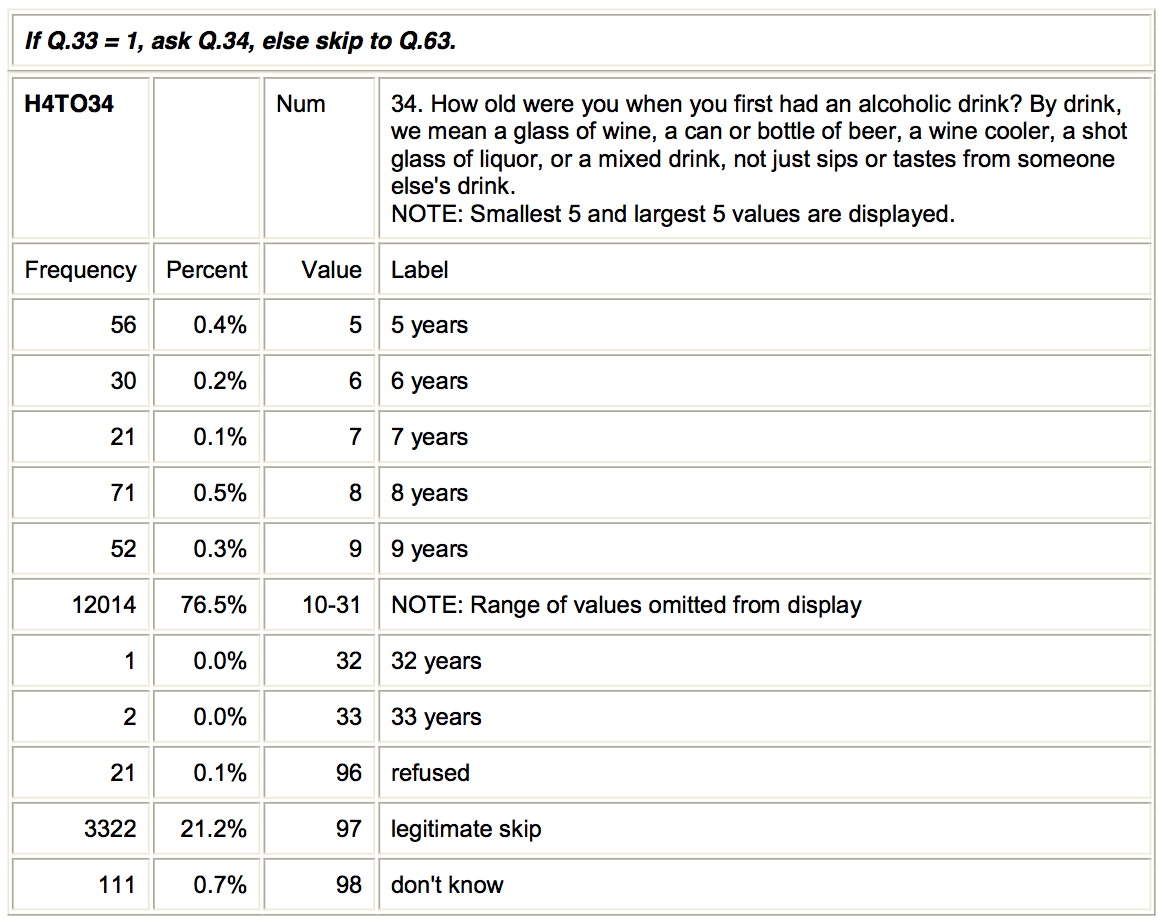
\includegraphics[width=3.5in]{h4to34_codebook.png}
      \end{center}
    \end{frame}

    \begin{frame}[fragile]
\begin{knitrout}
\definecolor{shadecolor}{rgb}{0.137, 0.137, 0.137}\begin{kframe}
\begin{alltt}
\hlstd{> }\hlstd{age} \hlkwb{<-} \hlstd{addhealth_public4}\hlopt{$}\hlstd{h4to34}
\hlstd{> }\hlstd{age[age} \hlopt{>=} \hlnum{96}\hlstd{]} \hlkwb{<-} \hlnum{NA}
\hlstd{> }\hlkwd{hist}\hlstd{(age,} \hlkwc{main}\hlstd{=}\hlstr{''}\hlstd{,} \hlkwc{xlab}\hlstd{=}\hlstr{''}\hlstd{,} \hlkwc{col}\hlstd{=}\hlstr{'orange'}\hlstd{)}
\end{alltt}
\end{kframe}
\input{/tmp/figures/unnamed-chunk-4-1.tikz}

\end{knitrout}
    \end{frame}

    \begin{frame}{Let's examine our variables}
      \begin{center}
        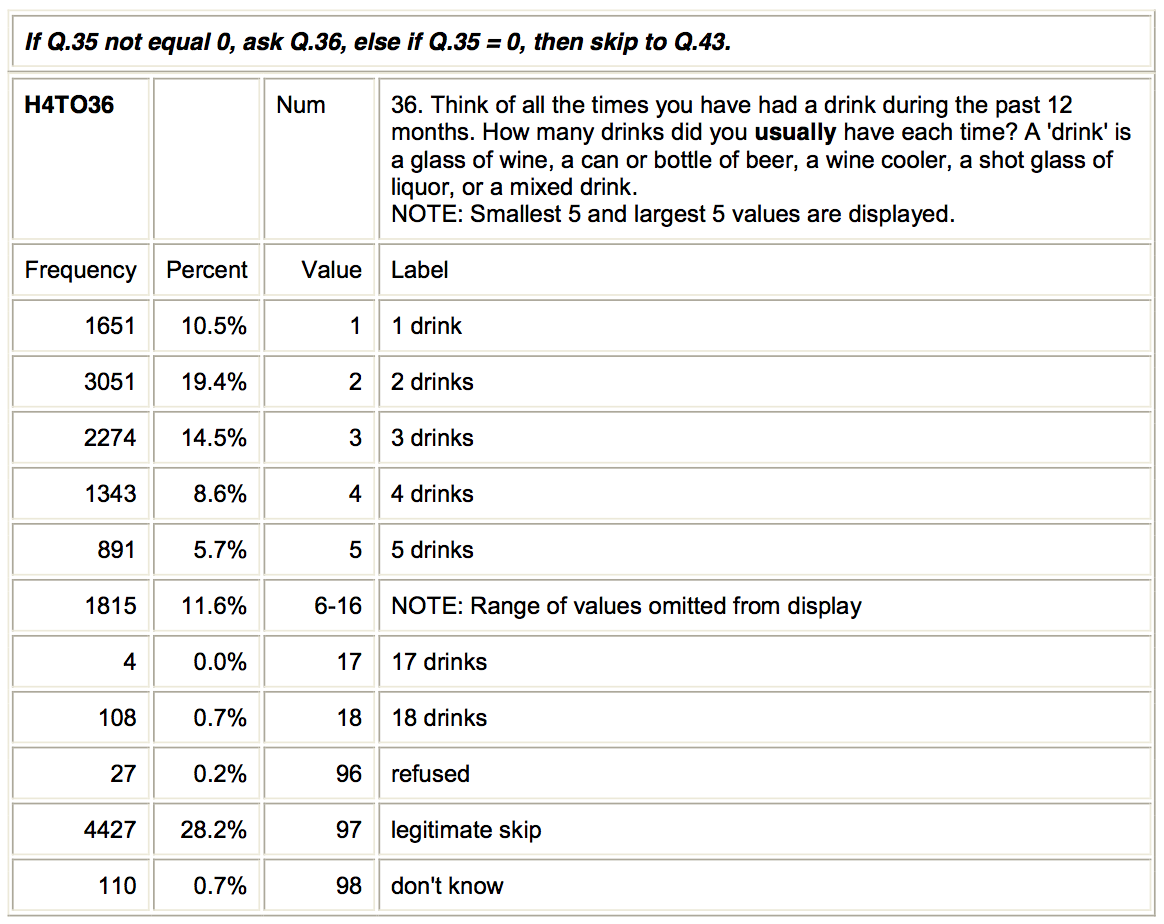
\includegraphics[width=3.5in]{h4to36_codebook.png}
      \end{center}
    \end{frame}

    \begin{frame}[fragile]
\begin{knitrout}
\definecolor{shadecolor}{rgb}{0.137, 0.137, 0.137}\begin{kframe}
\begin{alltt}
\hlstd{> }\hlstd{num.drinks} \hlkwb{<-} \hlstd{addhealth_public4}\hlopt{$}\hlstd{h4to36}
\hlstd{> }\hlstd{num.drinks[num.drinks} \hlopt{>=} \hlnum{96}\hlstd{]} \hlkwb{<-} \hlnum{NA}
\hlstd{> }\hlkwd{hist}\hlstd{(num.drinks,} \hlkwc{main}\hlstd{=}\hlstr{''}\hlstd{,} \hlkwc{xlab}\hlstd{=}\hlstr{'How many drinks'}\hlstd{,}
\hlstd{+ }  \hlkwc{col}\hlstd{=}\hlstr{'orange'}\hlstd{)}
\end{alltt}
\end{kframe}
\input{/tmp/figures/unnamed-chunk-5-1.tikz}

\end{knitrout}
    \end{frame}


    \begin{frame}[fragile]
\begin{knitrout}
\definecolor{shadecolor}{rgb}{0.137, 0.137, 0.137}\begin{kframe}
\begin{alltt}
\hlstd{> }\hlkwd{plot}\hlstd{(num.drinks} \hlopt{~} \hlstd{age,} \hlkwc{pch}\hlstd{=}\hlnum{16}\hlstd{,} \hlkwc{col}\hlstd{=}\hlstr{'orange'}\hlstd{,}
\hlstd{+ }  \hlkwc{xlab}\hlstd{=}\hlstr{'Age of first drink'}\hlstd{,}
\hlstd{+ }  \hlkwc{ylab}\hlstd{=}\hlstr{'Number of drinks consumed'}\hlstd{)}
\end{alltt}
\end{kframe}
\input{/tmp/figures/unnamed-chunk-6-1.tikz}

\end{knitrout}
    \end{frame}

    \begin{frame}[fragile]
\begin{knitrout}
\definecolor{shadecolor}{rgb}{0.137, 0.137, 0.137}\begin{kframe}
\begin{alltt}
\hlstd{> }\hlkwd{plot}\hlstd{(}\hlkwd{jitter}\hlstd{(num.drinks,} \hlnum{4}\hlstd{)} \hlopt{~} \hlkwd{jitter}\hlstd{(age,} \hlnum{4}\hlstd{),}
\hlstd{+ }  \hlkwc{pch}\hlstd{=}\hlnum{46}\hlstd{,} \hlkwc{col}\hlstd{=}\hlstr{'orange'}\hlstd{,}
\hlstd{+ }  \hlkwc{xlab}\hlstd{=}\hlstr{'Age of first drink'}\hlstd{,}
\hlstd{+ }  \hlkwc{ylab}\hlstd{=}\hlstr{'Number of drinks consumed'}\hlstd{)}
\end{alltt}
\end{kframe}
\input{/tmp/figures/unnamed-chunk-7-1.tikz}

\end{knitrout}
    \end{frame}

    \begin{frame}[fragile]
      The regression line is the line of ``best fit'' through this plot:
\begin{knitrout}
\definecolor{shadecolor}{rgb}{0.137, 0.137, 0.137}
\input{/tmp/figures/unnamed-chunk-8-1.tikz}

\end{knitrout}
      \lc
    \end{frame}

    \begin{frame}{What is linear regression doing?}
      We model each case ($x_i=$ age for $i$th person, $y_i=$ number of drinks for $i$th person) as a linear relationship plus some error:
      \[
        y_i = \beta_0 + \beta_1 x_i + \epsilon_i
      \]
      $\beta_0$ and $\beta_1$ are the intercept and slope, respectively.
      \bigskip\pause

      We find estimates for $\beta_0$ and $\beta_1$ in our sample that \emph{minimize} the errors:
      \[
        \hat Y = \hat\beta_0 + \hat\beta_1 X
      \]
      This is the regression (best fit) line.
    \end{frame}

    \begin{frame}[fragile]
      \fontsize{9}{9}\selectfont
\begin{knitrout}
\definecolor{shadecolor}{rgb}{0.137, 0.137, 0.137}\begin{kframe}
\begin{alltt}
\hlstd{> }\hlstd{model} \hlkwb{<-} \hlkwd{lm}\hlstd{(num.drinks} \hlopt{~} \hlstd{age)}
\hlstd{> }\hlkwd{summary}\hlstd{(model)}
\end{alltt}
\begin{verbatim}

Call:
lm(formula = num.drinks ~ age)

Residuals:
    Min      1Q  Median      3Q     Max 
-4.2035 -1.8528 -0.8528  0.8095 15.1602 

Coefficients:
            Estimate Std. Error t value Pr(>|t|)    
(Intercept)  6.55417    0.26532   24.70   <2e-16 ***
age         -0.16883    0.01588  -10.63   <2e-16 ***
---
Signif. codes:  0 '***' 0.001 '**' 0.01 '*' 0.05 '.' 0.1 ' ' 1

Residual standard error: 2.963 on 3600 degrees of freedom
  (2902 observations deleted due to missingness)
Multiple R-squared:  0.03044,	Adjusted R-squared:  0.03017 
F-statistic:   113 on 1 and 3600 DF,  p-value: < 2.2e-16
\end{verbatim}
\end{kframe}
\end{knitrout}
      \lc
    \end{frame}

    \begin{frame}[fragile]
      This translates to a regression line of:

      \[
        \widehat{\text{num drinks}} = 6.55 - 0.17 \cdot\text{age}
      \]
      \pause
      Predict number of drinks for $\text{age}=21$:
      \[
        \widehat{\text{num drinks}} 
        = 6.55 - 0.17 \cdot 21
        = 3.01
      \]
      Or we can use R to do the work for us:
\begin{knitrout}
\definecolor{shadecolor}{rgb}{0.137, 0.137, 0.137}\begin{kframe}
\begin{alltt}
\hlstd{> }\hlkwd{predict.lm}\hlstd{(model,} \hlkwd{list}\hlstd{(}\hlkwc{age}\hlstd{=}\hlnum{21}\hlstd{))}
\end{alltt}
\end{kframe}
\end{knitrout}
      \lc
    \end{frame}

    \begin{frame}{How good are our predictions?}
      $R^2$ quantifies how closely the model fits the data.
      \begin{itemize}[<+->]
        \item $R^2=\text{cor}(X,Y)^2$, i.e., the squared correlation between $X$ and $Y$.
        \item $R^2=0$ when the model has no predictive power at all.
        \item $R^2=1$ when the model yields perfect predictions every time.
        \item $R^2=\text{cor}(Y,\hat Y)^2$, i.e., the squared correlation between the actual and predicted values of $Y$.
      \end{itemize}
    \end{frame}

    \begin{frame}[fragile]
      \note{Point out where $R^2$ is found on the R output.}
      \fontsize{9}{9}\selectfont
\begin{knitrout}
\definecolor{shadecolor}{rgb}{0.137, 0.137, 0.137}\begin{kframe}
\begin{alltt}
\hlstd{> }\hlstd{model} \hlkwb{<-} \hlkwd{lm}\hlstd{(num.drinks} \hlopt{~} \hlstd{age)}
\hlstd{> }\hlkwd{summary}\hlstd{(model)}
\end{alltt}
\begin{verbatim}

Call:
lm(formula = num.drinks ~ age)

Residuals:
   Min     1Q Median     3Q    Max 
-4.204 -1.853 -0.853  0.810 15.160 

Coefficients:
            Estimate Std. Error t value Pr(>|t|)    
(Intercept)   6.5542     0.2653    24.7   <2e-16 ***
age          -0.1688     0.0159   -10.6   <2e-16 ***
---
Signif. codes:  0 '***' 0.001 '**' 0.01 '*' 0.05 '.' 0.1 ' ' 1

Residual standard error: 3 on 3600 degrees of freedom
  (2902 observations deleted due to missingness)
Multiple R-squared:  0.0304,	Adjusted R-squared:  0.0302 
F-statistic:  113 on 1 and 3600 DF,  p-value: <2e-16
\end{verbatim}
\end{kframe}
\end{knitrout}
    \end{frame} 

    \begin{frame}
      In our regression, $R^2=0.03$, so $r=\sqrt{0.03}=0.17$.  

      Is this ``significant?''
      \pause
      \begin{itemize}[<+->]
        \item \textbf{Statistical significance:} Can we reject the null hypothesis that the correlation between $X$ and $Y$ in the \emph{population} is not zero?
        \item \textbf{Practical significance:} Is the correlation in our sample large enough to be meaningful?
      \end{itemize}
    \end{frame}

    \begin{frame}{The overall null hypothesis for a regression model}
      The following are equivalent ways to express the overall null hypothesis:
      \begin{itemize}[<+->]
        \item $R^2=0$ (in the population)
        \item $\text{cor}(X,Y)=0$ (in the population)
        \item $\beta_1=0$
        \item The model has no predictive power
        \item Predictions from this model are no better than predicting $\overline Y$ for every case
      \end{itemize}
    \end{frame}

    \begin{frame}{Two ways to test the overall null hypothesis}
      \begin{itemize}
        \item The $F$-test (tests $H_0:R^2=0$ in the population)
        \item The $t$-test for the \emph{slope} ($\beta_1$) coefficient (tests $H_0:\beta_1=0$)
      \end{itemize}
      \pause
      Both of these methods are equivalent; the $p$-values will be exactly the same!
    \end{frame}

    \begin{frame}[fragile]
      \note{Point out where these $p$-values are found on the R output.}
      \fontsize{9}{9}\selectfont
\begin{knitrout}
\definecolor{shadecolor}{rgb}{0.137, 0.137, 0.137}\begin{kframe}
\begin{alltt}
\hlstd{> }\hlstd{model} \hlkwb{<-} \hlkwd{lm}\hlstd{(num.drinks} \hlopt{~} \hlstd{age)}
\hlstd{> }\hlkwd{summary}\hlstd{(model)}
\end{alltt}
\begin{verbatim}

Call:
lm(formula = num.drinks ~ age)

Residuals:
   Min     1Q Median     3Q    Max 
-4.204 -1.853 -0.853  0.810 15.160 

Coefficients:
            Estimate Std. Error t value Pr(>|t|)    
(Intercept)   6.5542     0.2653    24.7   <2e-16 ***
age          -0.1688     0.0159   -10.6   <2e-16 ***
---
Signif. codes:  0 '***' 0.001 '**' 0.01 '*' 0.05 '.' 0.1 ' ' 1

Residual standard error: 3 on 3600 degrees of freedom
  (2902 observations deleted due to missingness)
Multiple R-squared:  0.0304,	Adjusted R-squared:  0.0302 
F-statistic:  113 on 1 and 3600 DF,  p-value: <2e-16
\end{verbatim}
\end{kframe}
\end{knitrout}
    \end{frame}

    \begin{frame}{What is our conclusion about $\beta_1$?}
      \begin{itemize}[<+->]
        \item There is a \textbf{statistically significant} relationship between the age someone starts drinking and how much they drink as an adult.
        \item Or: People that start drinking earlier in life consume \textbf{significantly more} alcohol when they drink as adults.
        \item Each additional year you wait to start drinking is associated with consuming 0.17 fewer drinks as an adult.
        \item Is this relationship \textbf{practically significant}?
      \end{itemize}
    \end{frame}

    \begin{frame}{Put a confidence interval on it}
      \begin{itemize}[<+->]
        \item Our best estimate for the \emph{effect} of a year's postponement of drinking is 0.17 fewer drinks as an adult
        \item We can use a confidence interval to give a range of plausible values for what this effect size is in the population 
      \end{itemize}
    \end{frame}

    \begin{frame}[fragile]{Put a confidence interval on it}
      A confidence interval is always of the form \[ \text{estimate} \pm (\text{critical value})(\text{standard error}). \]
      \pause
      Recall that the critical value for a 95\% confidence interval is the cutoff value that cuts off 95\% of the area in the middle of the distribution; the sampling distribution of $\hat\beta_1$ is a $t$-distribution.


\begin{knitrout}
\definecolor{shadecolor}{rgb}{0.137, 0.137, 0.137}\begin{kframe}
\begin{alltt}
\hlstd{> }\hlstd{n} \hlkwb{<-} \hlkwd{nobs}\hlstd{(model)}
\hlstd{> }\hlkwd{qt}\hlstd{(}\hlnum{0.975}\hlstd{, n}\hlopt{-}\hlnum{2}\hlstd{)}
\end{alltt}
\begin{verbatim}
[1] 1.960623
\end{verbatim}
\end{kframe}
\end{knitrout}
    \end{frame}

    \begin{frame}[fragile]{Put a confidence interval on it}
      R will also calculate confidence intervals for us:
\begin{knitrout}
\definecolor{shadecolor}{rgb}{0.137, 0.137, 0.137}\begin{kframe}
\begin{alltt}
\hlstd{> }\hlkwd{confint}\hlstd{(model)}
\end{alltt}
\begin{verbatim}
                 2.5 %     97.5 %
(Intercept)  6.0339847  7.0743549
age         -0.1999713 -0.1376959
\end{verbatim}
\end{kframe}
\end{knitrout}

      \pause
      In other words, we are 95\% confident that the effect of each additional year's delay in starting to drink is between 0.14 and 0.2.
    \end{frame}

    \begin{frame}{Put a confidence interval on it, part 2}
      We can also put a confidence interval on a prediction!  

      Two kinds of intervals:
      \bigskip

      \begin{tabular}{lp{1in}p{2in}}
        \textbf{Confidence} & Predicting the mean value of $Y$ for a particular $X$. & Among all people that start drinking at age 21, how many drinks do have on average as adults? \\
        \textbf{Prediction} & Predicting $Y$ for a single new case. & If Bob started drinking at age 21, how many drinks do we think will have as an adult? \\
      \end{tabular}
    \end{frame}

    \begin{frame}[fragile]{Put a confidence interval on it, part 2}

\begin{knitrout}
\definecolor{shadecolor}{rgb}{0.137, 0.137, 0.137}\begin{kframe}
\begin{alltt}
\hlstd{> }\hlkwd{predict.lm}\hlstd{(model,} \hlkwd{list}\hlstd{(}\hlkwc{age}\hlstd{=}\hlnum{21}\hlstd{),}
\hlstd{+ }  \hlkwc{interval}\hlstd{=}\hlstr{'confidence'}\hlstd{)}
\end{alltt}
\begin{verbatim}
       fit     lwr      upr
1 3.008664 2.83616 3.181167
\end{verbatim}
\begin{alltt}
\hlstd{> }\hlkwd{predict.lm}\hlstd{(model,} \hlkwd{list}\hlstd{(}\hlkwc{age}\hlstd{=}\hlnum{21}\hlstd{),}
\hlstd{+ }  \hlkwc{interval}\hlstd{=}\hlstr{'prediction'}\hlstd{)}
\end{alltt}
\begin{verbatim}
       fit       lwr      upr
1 3.008664 -2.802894 8.820221
\end{verbatim}
\end{kframe}
\end{knitrout}

      \pause
      Why is the prediction interval wider?
      \lc
    \end{frame}

  \end{darkframes}

\end{document}
